% Options for packages loaded elsewhere
\PassOptionsToPackage{unicode}{hyperref}
\PassOptionsToPackage{hyphens}{url}
%
\documentclass[
  english,
  man,floatsintext]{apa6}
\usepackage{lmodern}
\usepackage{amssymb,amsmath}
\usepackage{ifxetex,ifluatex}
\ifnum 0\ifxetex 1\fi\ifluatex 1\fi=0 % if pdftex
  \usepackage[T1]{fontenc}
  \usepackage[utf8]{inputenc}
  \usepackage{textcomp} % provide euro and other symbols
\else % if luatex or xetex
  \usepackage{unicode-math}
  \defaultfontfeatures{Scale=MatchLowercase}
  \defaultfontfeatures[\rmfamily]{Ligatures=TeX,Scale=1}
\fi
% Use upquote if available, for straight quotes in verbatim environments
\IfFileExists{upquote.sty}{\usepackage{upquote}}{}
\IfFileExists{microtype.sty}{% use microtype if available
  \usepackage[]{microtype}
  \UseMicrotypeSet[protrusion]{basicmath} % disable protrusion for tt fonts
}{}
\makeatletter
\@ifundefined{KOMAClassName}{% if non-KOMA class
  \IfFileExists{parskip.sty}{%
    \usepackage{parskip}
  }{% else
    \setlength{\parindent}{0pt}
    \setlength{\parskip}{6pt plus 2pt minus 1pt}}
}{% if KOMA class
  \KOMAoptions{parskip=half}}
\makeatother
\usepackage{xcolor}
\IfFileExists{xurl.sty}{\usepackage{xurl}}{} % add URL line breaks if available
\IfFileExists{bookmark.sty}{\usepackage{bookmark}}{\usepackage{hyperref}}
\hypersetup{
  pdftitle={Lab 9 Example papaja},
  pdfauthor={Cory K. Costello1},
  pdflang={en-EN},
  pdfkeywords={Example, papaja, reproducible reporting},
  hidelinks,
  pdfcreator={LaTeX via pandoc}}
\urlstyle{same} % disable monospaced font for URLs
\usepackage{graphicx,grffile}
\makeatletter
\def\maxwidth{\ifdim\Gin@nat@width>\linewidth\linewidth\else\Gin@nat@width\fi}
\def\maxheight{\ifdim\Gin@nat@height>\textheight\textheight\else\Gin@nat@height\fi}
\makeatother
% Scale images if necessary, so that they will not overflow the page
% margins by default, and it is still possible to overwrite the defaults
% using explicit options in \includegraphics[width, height, ...]{}
\setkeys{Gin}{width=\maxwidth,height=\maxheight,keepaspectratio}
% Set default figure placement to htbp
\makeatletter
\def\fps@figure{htbp}
\makeatother
\setlength{\emergencystretch}{3em} % prevent overfull lines
\providecommand{\tightlist}{%
  \setlength{\itemsep}{0pt}\setlength{\parskip}{0pt}}
\setcounter{secnumdepth}{-\maxdimen} % remove section numbering
% Make \paragraph and \subparagraph free-standing
\ifx\paragraph\undefined\else
  \let\oldparagraph\paragraph
  \renewcommand{\paragraph}[1]{\oldparagraph{#1}\mbox{}}
\fi
\ifx\subparagraph\undefined\else
  \let\oldsubparagraph\subparagraph
  \renewcommand{\subparagraph}[1]{\oldsubparagraph{#1}\mbox{}}
\fi
% Manuscript styling
\usepackage{upgreek}
\captionsetup{font=singlespacing,justification=justified}

% Table formatting
\usepackage{longtable}
\usepackage{lscape}
% \usepackage[counterclockwise]{rotating}   % Landscape page setup for large tables
\usepackage{multirow}		% Table styling
\usepackage{tabularx}		% Control Column width
\usepackage[flushleft]{threeparttable}	% Allows for three part tables with a specified notes section
\usepackage{threeparttablex}            % Lets threeparttable work with longtable

% Create new environments so endfloat can handle them
% \newenvironment{ltable}
%   {\begin{landscape}\begin{center}\begin{threeparttable}}
%   {\end{threeparttable}\end{center}\end{landscape}}
\newenvironment{lltable}{\begin{landscape}\begin{center}\begin{ThreePartTable}}{\end{ThreePartTable}\end{center}\end{landscape}}

% Enables adjusting longtable caption width to table width
% Solution found at http://golatex.de/longtable-mit-caption-so-breit-wie-die-tabelle-t15767.html
\makeatletter
\newcommand\LastLTentrywidth{1em}
\newlength\longtablewidth
\setlength{\longtablewidth}{1in}
\newcommand{\getlongtablewidth}{\begingroup \ifcsname LT@\roman{LT@tables}\endcsname \global\longtablewidth=0pt \renewcommand{\LT@entry}[2]{\global\advance\longtablewidth by ##2\relax\gdef\LastLTentrywidth{##2}}\@nameuse{LT@\roman{LT@tables}} \fi \endgroup}

% \setlength{\parindent}{0.5in}
% \setlength{\parskip}{0pt plus 0pt minus 0pt}

% \usepackage{etoolbox}
\makeatletter
\patchcmd{\HyOrg@maketitle}
  {\section{\normalfont\normalsize\abstractname}}
  {\section*{\normalfont\normalsize\abstractname}}
  {}{\typeout{Failed to patch abstract.}}
\patchcmd{\HyOrg@maketitle}
  {\section{\protect\normalfont{\@title}}}
  {\section*{\protect\normalfont{\@title}}}
  {}{\typeout{Failed to patch title.}}
\makeatother
\shorttitle{lab 9}
\keywords{Example, papaja, reproducible reporting\newline\indent Word count: X}
\usepackage{csquotes}
\usepackage{setspace}
\AtBeginEnvironment{tabular}{\singlespacing}
\AtBeginEnvironment{lltable}{\singlespacing}
\AtBeginEnvironment{tablenotes}{\doublespacing}
\captionsetup[table]{font={stretch=1.5}}
\captionsetup[figure]{font={stretch=1.5}}
\ifxetex
  % Load polyglossia as late as possible: uses bidi with RTL langages (e.g. Hebrew, Arabic)
  \usepackage{polyglossia}
  \setmainlanguage[]{english}
\else
  \usepackage[shorthands=off,main=english]{babel}
\fi

\title{Lab 9 Example papaja}
\author{Cory K. Costello\textsuperscript{1}}
\date{}


\authornote{

Cory K. Costello, University of Oregon, Department of Psychology, 1227 University of Oregon, Eugene, OR, 97403

Correspondence concerning this article should be addressed to Cory K. Costello, Department of Psychology, 1227 University of Oregon, Eugene, OR, 97403. E-mail: \href{mailto:ccostell@uoregon.edu}{\nolinkurl{ccostell@uoregon.edu}}

}

\affiliation{\vspace{0.5cm}\textsuperscript{1} University of Oregon}

\abstract{
One or two sentences providing a \textbf{basic introduction} to the field, comprehensible to a scientist in any discipline.

Two to three sentences of \textbf{more detailed background}, comprehensible to scientists in related disciplines.

One sentence clearly stating the \textbf{general problem} being addressed by this particular study.

One sentence summarizing the main result (with the words ``\textbf{here we show}'' or their equivalent).

Two or three sentences explaining what the \textbf{main result} reveals in direct comparison to what was thought to be the case previously, or how the main result adds to previous knowledge.

One or two sentences to put the results into a more \textbf{general context}.

Two or three sentences to provide a \textbf{broader perspective}, readily comprehensible to a scientist in any discipline.
}



\begin{document}
\maketitle

We could start our introduction here, potentially saying something about the history of the Big Five (Goldberg, 1990), or about Roberts and colleagues' (2005). We could also mention McClelland and Judd (1993).

\hypertarget{methods}{%
\section{Methods}\label{methods}}

We report how we determined our sample size, all data exclusions (if any), all manipulations, and all measures in the study.

\hypertarget{participants}{%
\subsection{Participants}\label{participants}}

We have 2800 participants who completed some or all of the Big Five.

\hypertarget{material}{%
\subsection{Material}\label{material}}

\hypertarget{procedure}{%
\subsection{Procedure}\label{procedure}}

\hypertarget{data-analysis}{%
\subsection{Data analysis}\label{data-analysis}}

We used R (Version 4.0.2; R Core Team, 2019) and the R-packages \emph{corx} (Version 1.0.6.1; Conigrave, 2019), \emph{dplyr} (Version 1.0.2; Wickham et al., 2020), \emph{forcats} (Version 0.5.0; Wickham, 2020), \emph{ggplot2} (Version 3.3.2; Wickham, 2016), \emph{papaja} (Version 0.1.0.9997; Aust \& Barth, 2018), \emph{purrr} (Version 0.3.4; Henry \& Wickham, 2019), \emph{readr} (Version 1.4.0; Wickham, Hester, \& Francois, 2018), \emph{stringr} (Version 1.4.0; Wickham, 2019), \emph{tibble} (Version 3.0.4; Müller \& Wickham, 2019), \emph{tidyr} (Version 1.1.2; Wickham \& Henry, 2020), and \emph{tidyverse} (Version 1.3.0; Wickham, Averick, et al., 2019) for all our analyses.

\hypertarget{results}{%
\section{Results}\label{results}}

\begin{table}[tbp]

\begin{center}
\begin{threeparttable}

\caption{\label{tab:descrips-tab}Descriptive statistics of Big Five Scale Scores.}

\begin{tabular}{llllll}
\toprule
scale & \multicolumn{1}{c}{Mean} & \multicolumn{1}{c}{Median} & \multicolumn{1}{c}{SD} & \multicolumn{1}{c}{Min} & \multicolumn{1}{c}{Max}\\
\midrule
agree & 4.65 & 4.80 & 0.90 & 1.00 & 6.00\\
conscientious & 4.27 & 4.40 & 0.95 & 1.00 & 6.00\\
extraversion & 4.15 & 4.20 & 1.06 & 1.00 & 6.00\\
neuroticism & 3.16 & 3.00 & 1.20 & 1.00 & 6.00\\
openness & 4.59 & 4.60 & 0.81 & 1.20 & 6.00\\
\bottomrule
\addlinespace
\end{tabular}

\begin{tablenotes}[para]
\normalsize{\textit{Note.} This table was created with apa\_table().}
\end{tablenotes}

\end{threeparttable}
\end{center}

\end{table}

\begin{table}[tbp]

\begin{center}
\begin{threeparttable}

\caption{\label{tab:scale-intercors-tbl}Example corr matrix}

\begin{tabular}{lllll}
\toprule
 & \multicolumn{1}{c}{1} & \multicolumn{1}{c}{2} & \multicolumn{1}{c}{3} & \multicolumn{1}{c}{4}\\
\midrule
1. agree & - &  &  & \\
2. conscientious & .26*** & - &  & \\
3. extraversion & .46*** & .26*** & - & \\
4. neuroticism & -.19*** & -.23*** & -.22*** & -\\
5. openness & .15*** & .20*** & .21*** & -.09***\\
\bottomrule
\addlinespace
\end{tabular}

\begin{tablenotes}[para]
\normalsize{\textit{Note.} * p < 0.05; ** p < 0.01; *** p < 0.001}
\end{tablenotes}

\end{threeparttable}
\end{center}

\end{table}

\begin{table}[tbp]

\begin{center}
\begin{threeparttable}

\caption{\label{tab:reg-models-tbl}Regressing Conscientiousness on Age and Education}

\begin{tabular}{lll}
\toprule
 & \multicolumn{1}{c}{Model 1} & \multicolumn{1}{c}{Model 2}\\
\midrule
Intercept & $4.30$ $[4.26$, $4.33]$ & $4.16$ $[4.03$, $4.28]$\\
Age & $0.01$ $[0.00$, $0.01]$ & $0.01$ $[0.01$, $0.01]$\\
Education College Grad &  & $0.02$ $[-0.13$, $0.18]$\\
Education Finished HS &  & $0.05$ $[-0.12$, $0.21]$\\
Education Grad Degree &  & $0.06$ $[-0.09$, $0.22]$\\
Education Some College &  & $0.25$ $[0.11$, $0.38]$\\
$R^2$ [90\% CI] & $.01$ $[0.00$, $0.02]$ & $.02$ $[0.01$, $0.03]$\\
$F$ & 22.16 & 10.93\\
$df_1$ & 1 & 5\\
$df_2$ & 2575 & 2571\\
$p$ & < .001 & < .001\\
$\mathrm{AIC}$ & 6,979.81 & 6,955.69\\
$\mathrm{BIC}$ & 6,997.38 & 6,996.68\\
$\Delta R^2$ &  & $.01$\\
$F$ &  & 8.06\\
$df_1$ &  & 4\\
$df_2$ &  & 2,575\\
$p$ &  & < .001\\
$\Delta \mathrm{AIC}$ &  & -24.12\\
$\Delta \mathrm{BIC}$ &  & -0.70\\
\bottomrule
\addlinespace
\end{tabular}

\begin{tablenotes}[para]
\normalsize{\textit{Note.} Model comparison compares a model with just age to a model that has age and education.}
\end{tablenotes}

\end{threeparttable}
\end{center}

\end{table}



\begin{figure}
\centering
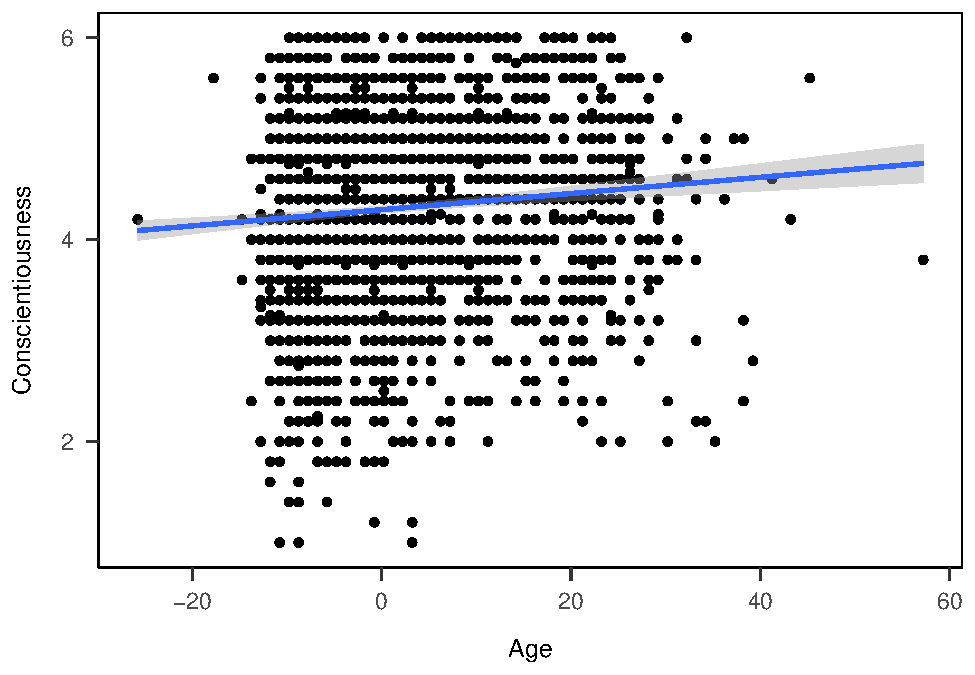
\includegraphics{papaja_example_ms_files/figure-latex/fig-ageXconsc-1.pdf}
\caption{\label{fig:fig-ageXconsc}Conscientiousness by Age.}
\end{figure}

We calculated scale scores for each of the Big Five. Descriptive statistics for each Big Five scale are shown in Table~\ref{tab:descrips-tab}, where it is apparent that means were near the scale midpoints of 4.5, with the exception of neuroticism which had a much lower mean of 3.13.

Scale inter-correlations can be found in Table~\ref{tab:scale-intercors-tbl}, where one can see that the smallest correlation was between neuroticism and opennes (\emph{r} = -0.09) and the largest correlation was between extraversion and agreeableness (\emph{r} = 0.46).

We next examined the extent to which grand-mean centered age and education are related to conscientiousness, based on the postulates of social investment theory (Roberts et al., 2005). The results from a model with just age and a model with age and education are shown in Table~\ref{tab:reg-models-tbl} below. Age had a small but significant, positive association with conscientiousness, both when education is (\(b = 0.01\), 95\% CI \([0.01\), \(0.01]\), \(t(2571) = 5.54\), \(p < .001\)) and is not (\(b = 0.01\), 95\% CI \([0.00\), \(0.01]\), \(t(2575) = 4.71\), \(p < .001\)) included as a covariate. Education did significantly but modestly improve the model (\(\Delta R^2 = .01\), \(F(4, 2,575) = 8.06\), \(p < .001\)). Interestingly, the pattern of results did not follow a monotonic increase from some highschool to graduate degree. Indeed, the only significant difference in conscientiousness across education was between participants who didn't finish high school and participants who reported having some college (\(b = 0.25\), 95\% CI \([0.11\), \(0.38]\), \(t(2571) = 3.63\), \(p < .001\)). At the sample average age, participants who didn't finish highschool had an average conscientiousness score of (\(M_{SomeHS}\) = 4.16) while participants with some college had an average conscientiousness score of (\(M_{SomeCollege}\) = 4.40). The remaining effects of education were small and non-significant (see Table~\ref{tab:reg-models-tbl}).

Figure~\ref{fig:fig-ageXconsc} depicts the small, linear increase of conscientiousness across the age range of our participants.

\hypertarget{discussion}{%
\section{Discussion}\label{discussion}}

\newpage

\hypertarget{references}{%
\section{References}\label{references}}

\begingroup
\setlength{\parindent}{-0.5in}
\setlength{\leftskip}{0.5in}

\hypertarget{refs}{}
\leavevmode\hypertarget{ref-R-papaja}{}%
Aust, F., \& Barth, M. (2018). \emph{papaja: Create APA manuscripts with R Markdown}. Retrieved from \url{https://github.com/crsh/papaja}

\leavevmode\hypertarget{ref-R-corx}{}%
Conigrave, J. (2019). \emph{Corx: Create and format correlation matrices}. Retrieved from \url{https://CRAN.R-project.org/package=corx}

\leavevmode\hypertarget{ref-goldberg1990alternative}{}%
Goldberg, L. R. (1990). An alternative" description of personality": The big-five factor structure. \emph{Journal of Personality and Social Psychology}, \emph{59}(6), 1216--1229. \url{https://doi.org/https://doi.org/10.1037/0022-3514.59.6.1216}

\leavevmode\hypertarget{ref-R-purrr}{}%
Henry, L., \& Wickham, H. (2019). \emph{Purrr: Functional programming tools}. Retrieved from \url{https://CRAN.R-project.org/package=purrr}

\leavevmode\hypertarget{ref-mcclelland1993statistical}{}%
McClelland, G. H., \& Judd, C. M. (1993). Statistical difficulties of detecting interactions and moderator effects. \emph{Psychological Bulletin}, \emph{114}(2), 376.

\leavevmode\hypertarget{ref-R-tibble}{}%
Müller, K., \& Wickham, H. (2019). \emph{Tibble: Simple data frames}. Retrieved from \url{https://CRAN.R-project.org/package=tibble}

\leavevmode\hypertarget{ref-R-base}{}%
R Core Team. (2019). \emph{R: A language and environment for statistical computing}. Vienna, Austria: R Foundation for Statistical Computing. Retrieved from \url{https://www.R-project.org/}

\leavevmode\hypertarget{ref-roberts2005}{}%
Roberts, B. W., Wood, D., \& Smith, J. L. (2005). Evaluating five factor theory and social investment perspectives on personality trait development. \emph{Journal of Research in Personality}, \emph{39}(1), 166--184.

\leavevmode\hypertarget{ref-R-ggplot2}{}%
Wickham, H. (2016). \emph{Ggplot2: Elegant graphics for data analysis}. Springer-Verlag New York. Retrieved from \url{https://ggplot2.tidyverse.org}

\leavevmode\hypertarget{ref-R-stringr}{}%
Wickham, H. (2019). \emph{Stringr: Simple, consistent wrappers for common string operations}. Retrieved from \url{https://CRAN.R-project.org/package=stringr}

\leavevmode\hypertarget{ref-R-forcats}{}%
Wickham, H. (2020). \emph{Forcats: Tools for working with categorical variables (factors)}. Retrieved from \url{https://CRAN.R-project.org/package=forcats}

\leavevmode\hypertarget{ref-R-tidyverse}{}%
Wickham, H., Averick, M., Bryan, J., Chang, W., McGowan, L. D., François, R., \ldots{} Yutani, H. (2019). Welcome to the tidyverse. \emph{Journal of Open Source Software}, \emph{4}(43), 1686. \url{https://doi.org/10.21105/joss.01686}

\leavevmode\hypertarget{ref-R-dplyr}{}%
Wickham, H., François, R., Henry, L., \& Müller, K. (2020). \emph{Dplyr: A grammar of data manipulation}. Retrieved from \url{https://CRAN.R-project.org/package=dplyr}

\leavevmode\hypertarget{ref-R-tidyr}{}%
Wickham, H., \& Henry, L. (2020). \emph{Tidyr: Tidy messy data}. Retrieved from \url{https://CRAN.R-project.org/package=tidyr}

\leavevmode\hypertarget{ref-R-readr}{}%
Wickham, H., Hester, J., \& Francois, R. (2018). \emph{Readr: Read rectangular text data}. Retrieved from \url{https://CRAN.R-project.org/package=readr}

\endgroup


\end{document}
